\documentclass{ltjsarticle}
\usepackage{amsmath}
\usepackage{amssymb}
\usepackage{ascmac}
\usepackage[dvipdfmx]{graphicx}
\usepackage{tabularx}
\usepackage[colorlinks=true, allcolors=blue]{hyperref}
\usepackage{fancybox}
\usepackage{tikz}
\usepackage{subcaption}
\usetikzlibrary{shapes,arrows}

\begin{document}

\title{103. 深層学習の適用方法(自然言語処理)}
\author{秋葉洋哉}
\maketitle

\section{Seq2Seq (Encoder-Decoder)}
\subsection{RNNと言語モデル}
Seq2seqとは、Sequence to Sequence の略であり、系列(Sequence)を入力として、系列を出力するものである。入力系列がEncode(=内部状態に変換)され、内部状態からDecode(=出力系列に変換)される。Seq2seqは、機械翻訳(英語-日本語)、音声認識(波形-テキスト)、質問応答システム(テキスト-テキスト)などに応用されている。
\par
Seq2Seqは、RNNと言語モデルを組み合わせたモデルである。RNNは、再帰型ニューラルネットワーク(Recurrent Neural Network)の略であり、図\ref{fig:RNN}のような構造を持つ。最終的に内部状態ベクトル$\mathbf{h}$を得ることが目的となる。
\begin{figure}[htbp]
  \centering
  \begin{subfigure}[b]{0.45\textwidth}
    \centering
    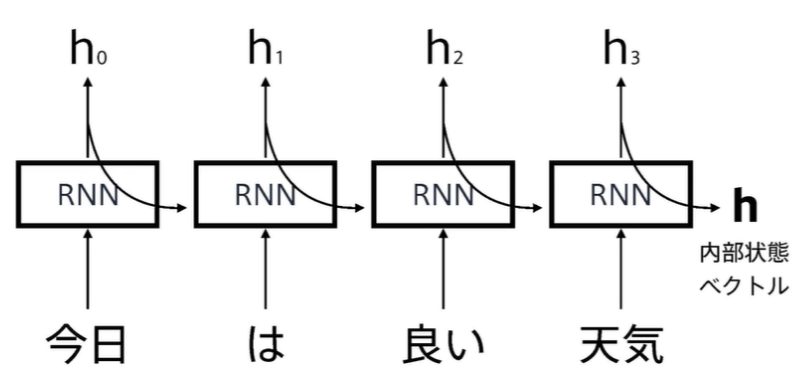
\includegraphics[width=0.8\linewidth]{./capture/RNN.png}
    \caption{RNNの構造: 最終的に内部状態ベクトル$\mathbf{h}$を得る。}
    \label{fig:RNN}
  \end{subfigure}
  \hfill
  \begin{subfigure}[b]{0.45\textwidth}
    \centering
    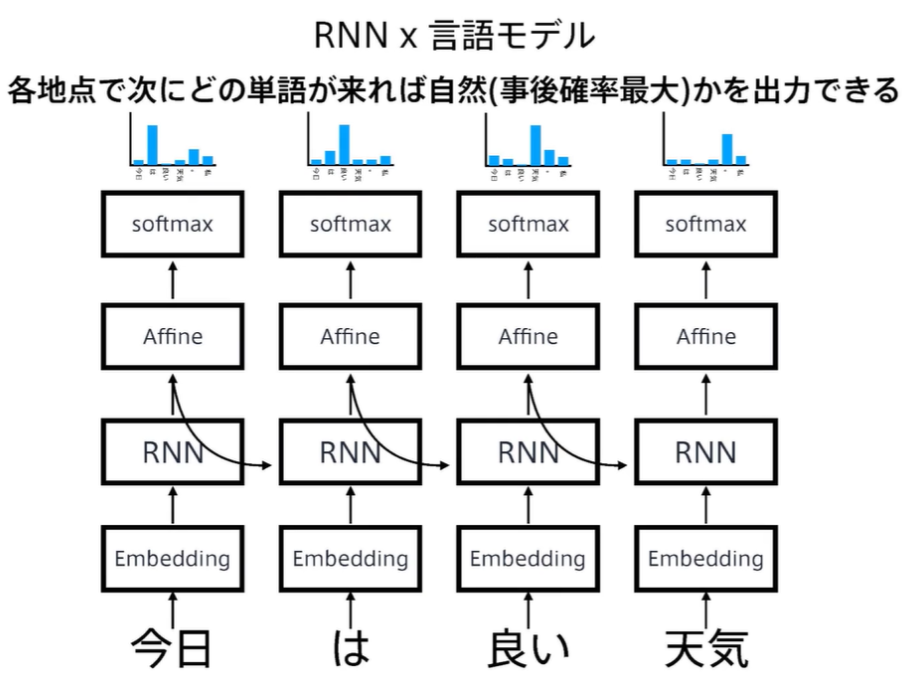
\includegraphics[width=0.8\linewidth]{./capture/RNN&LangModel.png}
    \caption{RNNと言語モデルを組み合わせた構造}
    \label{fig:RNN&LangModel}
  \end{subfigure}
  \caption{Seq2Seqの基本的な仕組み}
\end{figure}

言語モデルは、単語の並びに確率を与えるモデルであり、単語の並びに対してそれがどれだけ起こりうるか(尤度)、すなわち文章として自然かを確率で評価する。例えば、I am a student. という文章と、I student am a. という文章を比較すると、前者の方が自然であるため、言語モデルで出力される確率が高くなる。このような自然さを確率で評価するモデルを言語モデルと呼ぶ。RNNと言語モデルを組み合わせた時、図\ref{fig:RNN&LangModel}のような構造を持つことになる。
このモデルをEncoder、Decoderとして、内部状態ベクトル$h$を媒介して組み合わせたものがSeq2Seqである。

\subsection{Teacher Focing}
Seq2Seqでは、ひいてはRNNでは、予測を用いて次の予測を行うため、一つ間違えた時の影響が次々と伝播し、誤差が蓄積されてしまう。そこで、Decoderの入力に正解データを入力することで、学習を安定させることができる。この手法をTeacher Forcingと呼ぶ。本番時には、この手法は使えず、予測結果が次の入力となるため、誤差が蓄積されることに注意が必要となる。

\clearpage
\section{Transformer}
\subsection{概要}
Transformerは、Vaswani et al (2017) で提案されたモデルであり、Seq2Seqの問題点である長い系列を扱うことができる。
Transformerのアーキテクチャは図\ref{fig:Transformer}のように構成されており、RNNを用いず、代わりにAttention機構というモジュールが用いられる。
\begin{figure}[htbp]
  \centering
  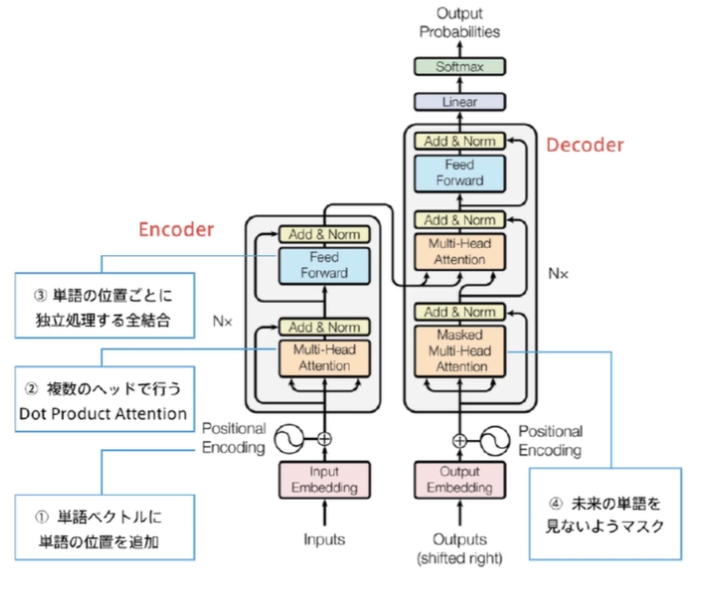
\includegraphics[width=10cm]{./capture/Transformer.png}
  \caption{Transformerのアーキテクチャ}
  \label{fig:Transformer}
\end{figure}

\subsection{Attention}
Transformerは、Attentionという機構を導入することで、長い系列を扱うことができる。Attentionは、入力系列の各要素に重みを付けることで、重要な要素に注目することができる。この機構を導入することで、長い系列を扱うことができるようになる。
\par
Attentionは辞書オブジェクトである。辞書オブジェクトとは、キーと値のペアを持つオブジェクトであり、キーを用いて値を取得することができる。Attentionは、Query、Key、Valueの3つの要素を持つ。Queryは、重要な要素を取得するためのキーであり、Keyは、入力系列の各要素のキーであり、Valueは、入力系列の各要素の値である。QueryとKeyの内積を取ることで、各要素の重要度を計算することができる。この重要度を用いて、Valueの重み付き和を計算することで、Attentionの出力を得ることができる。
\par
Attentionは、Source-Target-AttentionとSelf-Attentionの2つの種類がある。Source-Target-Attentionは、入力系列と出力系列の関係を表す。Self-Attentionは、入力系列の各要素に重みを付けることができる。

\subsection{Self-Attentionの計算}
Selt-Attentionの計算は、以下のように行われる(図\ref{fig:Self-Attention})。
\begin{enumerate}
  \item Query(正解のラベル)とKey(入力のラベル)の内積を計算する。すると、各要素の重要度が計算される。
  \item 効率的な逆伝播のために、内積をスケーリングする。\begin{math} \frac{QK^{T}}{\sqrt{d_k}} V \end{math}
  \item ソフトマックス関数を適用する。
  \item 3.の出力とValueの内積を計算する。
\end{enumerate}
これらの手順は、図\ref{fig:Transformer}の②に対応している。
図\ref{fig:Transformer}の④は、Decoderにおいて、

\begin{figure}[htbp]
  \centering
  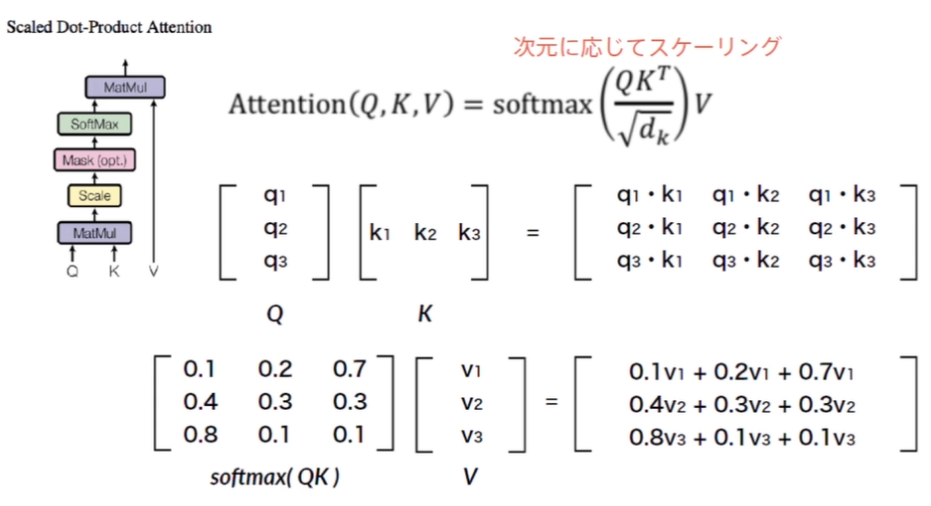
\includegraphics[width=10cm]{./capture/SelfAttention.png}
  \caption{Self-Attentionの計算}
  \label{fig:Self-Attention}
\end{figure}

\subsection{Add \& Norm}
Transformerでは、Self-Attentionの出力と入力を足し合わせることで、情報を保持する。その後、Layer Normalizationを行うことで、情報を正規化する。この手法は、ResNetでも用いられている手法であり、勾配消失問題を回避するために用いられる。

\subsection{Position Encoding}
Transformerは、Attention機構を用いるため、系列の順序情報を考慮することができない。そのため、Position Encodingという手法を用いて、系列の順序情報を考慮する。Position Encodingは、系列の各要素に対して、位置情報を付与する手法である。具体的には、各要素に対して、sin, cos関数を用いて、単語の位置情報を付与(エンコード)する。
この手法は、図\ref{fig:Transformer}の①に対応している。

\subsection{Masking}
TransformerのDecoderでは、未来の情報を見ないようにするために、Maskingという手法を用いる。この手法は、未来の情報を見ないようにするために、Attentionの重みを0にする手法である。
この手法は、図\ref{fig:Transformer}の④に対応している。

\subsection{Multi-Head Attention}
Multi-Head Attentionは、Self-Attentionをアンサンブルで用いる手法である。Self-Attentionを複数のヘッドに分割することで、複数の視点から情報を取得することができる。

\clearpage
\section{BLEU}
BLEUは、機械翻訳の評価指標の一つであり、Modified N-gram precisionを用いて、翻訳の正確さを評価する指標である。BLEUは、N-gramを用いて、翻訳の正確さを評価する。
\begin{align}
  \text{BLEU} = \text{BP} \times \exp\left( \sum_{n=1}^{N} w_n \log p_n \right)
\end{align}
ただし、BP(Brevity Penalty)は、短い文に($c<r$)対してペナルティを与えるための指標であり、$w_n$は、N-gramの重み、$p_n$は、Modified N-gram precisionである。
BPは以下で定義できる。
\begin{align}
  \text{BP} = \begin{cases}
    1 & \text{if } c > r \\
    \exp\left( 1 - \frac{r}{c} \right) & \text{if } c \leq r
  \end{cases}
\end{align}
ただし、$c$は、翻訳文の長さ、$r$は、参照文の長さである。
\par
$p_n$は、例を用いて説明する。以下のReference と Candidate があるとする。
\begin{align}
  \text{Reference} &= \text{the cat is on the mat} \\
  \text{Candidate:1} &= \text{the cate the on the mat}\\
  \text{Candidate:2} &= \text{the the the the the the the} \\
  \text{Candidate:3} &= \text{the cat are On The Mat}\\
\end{align}
この時のModified N-gram precisionの値は、
\begin{align}
  \text{Reference} &= \text{the cat is on the mat} : 5 \\
  \text{Candidate:1} &= \text{the cate the on the mat} : 2\\
  \text{Candidate:2} &= \text{the the the the the the the} : 0 \\
  \text{Candidate:3} &= \text{the cat are On The Mat} : 0\\
\end{align}
から、$(2+0+0)/5 = 2/5$と計算される。
\par
BLEUで対数加重平均で評価するメリットとしては、nが大きくなると、指数的にスコアが低くなってしまうのを平坦化することで、nが小さいときのスコアは、妥当性を評価し、nが大きいときのスコアは、流暢性を評価することができる。

\clearpage
\section{BERT}
BERTは、Bidirectional Encoder Representations from Transformersの略であり、2018年にGoogleによって提案されたモデルである。BERTは、Transformerをベースに開発されており、双方向の情報を考慮することができる。BERTは、Fine-Tuningアプローチの事前学習に工夫を加えることで、様々な自然言語処理のタスクに対応することができる。
\par
BERTは、以下のような特徴を持つ。
\begin{itemize}
  \item 双方向の情報を考慮することができる。
  \item 事前学習を行うことで、様々な自然言語処理のタスクに対応することができる。
  \item Attention機構を用いることで、長い系列を扱うことができる。
\end{itemize}

\clearpage
\section{GPT}
\subsection{概要}
GPTは、Generative Pre-trained Transformerの略であり、OpenAIによって提案されたモデルである。GPTは、巨大な文章のデータセット(約45TB)を用いて、事前学習を行い、パラメータ数は、1750億個にも達する(GPT-3の場合)。このおかげで、汎用的な特徴量を習得しており、手元の様々な新しいタスク(翻訳や質問応答など)に対して特化したデータセットの規模が小さくても、高精度で予測モデルを構築することができる。
\par
GPTの構造は、Transformerをベースとしているが、BERTと異なり、双方向の情報を考慮することができない。だが、BERTでは各タスクに対してファインチューニングが必要である一方で、GPT3は、ファインチューニングを必要としないにも関わらず、幅広い言語タスクを高精度で実行することができる(図\ref{fig:BERT_GPT})。
\begin{figure}[htbp]
  \centering
  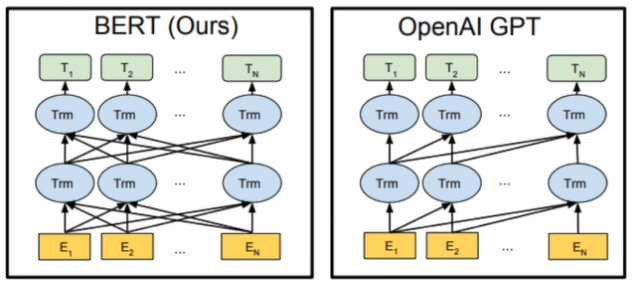
\includegraphics[width=12cm]{./capture/BERT_GPT.png}
  \caption{BERTとGPTの違い: BERTは文中のどの単語もマスクされる可能性があり、マスクした前の単語も後ろの単語にも注目する必要がある。一方で、GPTは常に次の単語を予測するため、双方向ではない。}
  \label{fig:BERT_GPT}
\end{figure}



\subsection{GPT-3の問題点}
まず、膨大な数のパラメータを使用するため、学習に多大なコストがかかる。
そして、モデルができたとしても、人間社会の慣習や常識を認識できないことで、不適切な回答をすることがある。特に、物理現象に関する推論を苦手としている。また、社会への課題も存在する。GPT-3は、人間らしい文章を生成する能力を有するため、フェイクニュースなどの悪用のリスクがある。

\subsection{GPTの事前学習}
GPTの事前学習では、以下の式を最大化する。
\begin{align}
  L_1(u) = \sum_i \log P(u_i | u_{i-k}, \cdots, u_{i-1}; \Theta)
\end{align}
ただし、$u$は、入力系列、$u_i$は、入力系列の$i$番目の要素、$\Theta$は、モデルのパラメータである。
$k$はコンテキストウィンドウのサイズであり、$u_i$を予測するために$u_i$の前にある$k$個の要素を考慮することを意味する。
学習は、以下の数式で表される。
\begin{align}
  h_0 = U W_e + W_p\\
  h_l = \text{TransformerBlock}(h_{l-1}) \quad \text{for } l = 1, \cdots, n\\
  P(u) = \text{softmax}(h_n W_e^T)
\end{align}
ただし、$U$は、対処の単語を予測するために使う$ u_{i-k}, \cdots, u_{i-1}$で、$W_e$は、単語の埋め込み行列、$W_p$は、位置エンコーディング行列、$h_l$は、$l$番目のTransformerブロックの出力、$n$は、Transformerブロックの数である。

GPTはTransformerのDecoderのみを用いている(図\ref{fig:GPT})。TransformerのDecoderと比較すると、Multi-Head Attention部分が減っただけの構造になっていることがわかる(図\ref{fig:Transformer})。
\begin{figure}[htbp]
  \centering
  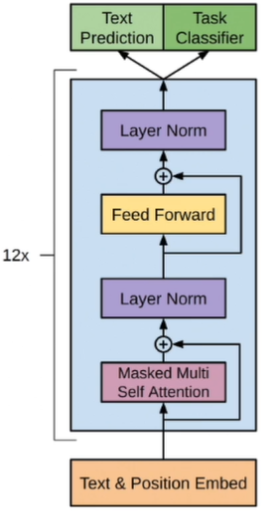
\includegraphics[width=5cm]{./capture/GPT.png}
  \caption{GPTの構造}
  \label{fig:GPT}
\end{figure}

\subsection{GPT-1のファインチューニング}
GPT-2, GPT-3で細かい変更があるものの、基本的な構造はGPT-1と同じである。GPT-1のファインチューニングは、始まりを表す記号、文と文を区切る記号、文の終わりを表す記号を用いる。
図\ref{fig:GPT-1_fine_tuning}は、上から順にテキスト分類タスク、文同士の関係予測タスク、文と文の類似度予測タスク、複数の文から一つを選ぶタスクを表している。
\begin{figure}[htbp]
  \centering
  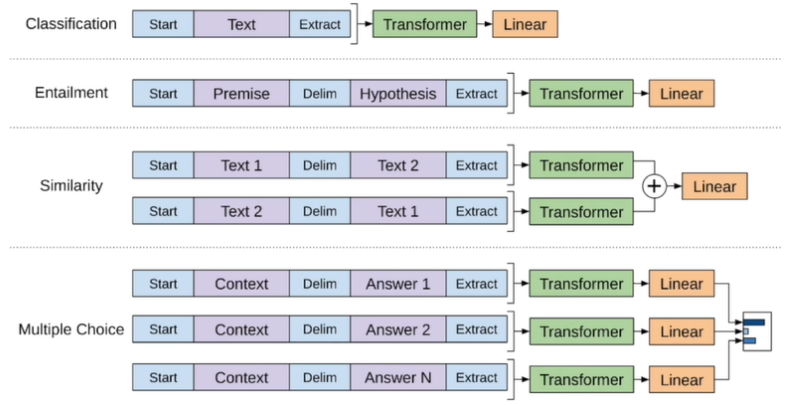
\includegraphics[width=10cm]{./capture/GPT-1_fine_tuning.png}
  \caption{GPT-1のファインチューニング}
  \label{fig:GPT-1_fine_tuning}
\end{figure}

\subsection{GPT-3の推論方法}
GPT-3の推論は、以下のように分類できる。
\begin{itemize}
  \item zero-shot: 何のタスクかを指定した後、すぐに推論させる方法 [入力例: 英語からフランス語へ翻訳してください。cheese]
  \item one-shot: 一度だけラベル付きの例を教え、その後に推論させる方法 [入力例: 英語からフランス語へ翻訳してください。sea otter => loutre de mer, cheese =>]
  \item few-shot: 2つ以上の例を教えた後、推論させる方法 [入力例: 英語からフランス語へ翻訳してください。sea otter => loutre de mer, plush girafe => girafe peluche, cheese =>]
\end{itemize}






\clearpage
\paragraph{参考文献}
\begin{enumerate}
  \item 岡谷貴之/深層学習 改訂第2版 [機械学習プロフェッショナルシリーズ]/ 講談社サイエンティフィク/ 2022-01-17
\end{enumerate}

\clearpage
\section{実装演習キャプチャ}
%------------
%Seq2Seq
%------------
\subsection{Seq2Seq}
\begin{figure}[htbp]
  \centering
  \includegraphics[width=10cm]{C:/Users/hiroh/Videos/Captures/4_1_transfer-learning/Arc 2024_07_04 22_00_53.png}
\end{figure}


\newpage
\end{document}